% homework/hw13/hw13.tex
% Year 7 - Homework Packet 13: Count It, Measure It, Key It.
%
% Maths 7.1 Part 1 (equivalent fractions, improper fractions and mixed
% numbers) at full Year 7 stretch; Maths 6.1 kinds of data, all from animals;
% Science 4.4 (using keys) and 4.5 (constructing keys). The teacher asked
% (17 Nov 2026) for eight pages, no French, "a section on organizing data into
% categorical, discrete, and continuous that relates to animals" that segues
% into "creating a dichotomous key for a set of animals".
%   Part 1  Section A. Fractions: equivalent chains, = or not equal with a
%           reason, improper <-> mixed with bigger numbers, "change it first",
%           word problems, Mr Bowen's homework, and calculation -> English.
%   Part 2  Section B. One data table of six animals from Viet Nam. Sort its
%           columns into the three kinds; the hard cases; a grouped frequency
%           table of baby crocodiles; and the bridge: a good key question asks
%           about something you can count, measure or see (4.5's write panel)
%           -- i.e. discrete, continuous or categorical data.
%   Part 3  Section C. Use a numbered key (sea animals); build a dichotomous
%           key for the six animals of B1, as a tree and then numbered; test
%           it; the elephant the key cannot name.
% English only (no French copy, at the teacher's request).
%
% Nothing untaught:
%   * 7.1 Part 1 (U07_1a): numerator / denominator; equivalent = multiply or
%     divide top and bottom by the same number; = and its not-equal sign;
%     improper -> mixed: divide, remainder on top; mixed -> improper: multiply
%     then add; "change it first" to compare an improper fraction with a
%     mixed number. Ordering fractions with different denominators is Part 2
%     (U07_1b, not taught yet), so A4(c) is made fair by "change both to
%     sixths".
%   * 6.1 (U06_1): data, categorical (a word), discrete (count), continuous
%     (measure); critique and suggest; grouped frequency table in equal groups
%     like 16.0-16.9; "is there evidence?".
%   * 4.4 (U04_4): key, dichotomous, the numbered style (1a / 1b, go to),
%     "a key can only identify the organisms that are in it".
%   * 4.5 (U04_5): a good key question (same answer from everyone: count,
%     measure or see); bad made good with -er than + a number; split into two,
%     split again, stop when each has its own name; test and fix.
%   * No animal from the decks (crab, dragonfly, housefly, earthworm, slug,
%     the four fish, the four cats, tiger, saola) and none of HW 12's gecko.
%     No number from the Workbook.
%
% Animal data are rounded, typical adult values (sun bear 120-150 cm and
% 27-80 kg, 1-2 cubs; water buffalo 240-300 cm and 300-1200 kg, 1 calf; Sunda
% pangolin about 90 cm with its tail and 2-7 kg, 1 baby; king cobra 3-4 m and
% about 6 kg, 20-40 eggs; common kingfisher 17 cm and about 40 g, 6-7 eggs;
% Siamese crocodile 2-3.5 m and 40-70 kg, 20-50 eggs). The packet says
% "about" and "an adult".
%
% House style is shared: see homework/hw-style.tex. Method: the new-homework
% skill. Source is pure ASCII on purpose.
%
% Build:  pwsh .claude/skills/new-homework/scripts/build-hw.ps1 hw13

\documentclass[12pt,a4paper]{article}

% -- Answer key switch -------------------------------------------------------
\newif\ifkey
\ifdefined\TEACHER\keytrue\else
  \keyfalse        % \keyfalse = student copy   |   \keytrue = teacher copy
\fi

% -- House style -------------------------------------------------------------
% homework/hw-style.tex
% Shared house style for every Year 7 homework packet. \input this from the
% packet file, right after \documentclass and the answer-key switch.
%
% Do not fork this file per packet. If a packet needs a different look, the
% question is whether every packet should have it.
%
% The choices here are deliberate and were arrived at by printing and looking:
%   * No solid dark banners. Every header is a light tint with a coloured spine
%     on the left, so colour reads clearly without flooding a school printer.
%   * No marks and no mark totals. These are practice, not exam papers.
%   * Lato at 12pt with open leading, plus mathastext so inline maths is Lato
%     too. Without mathastext every "-6 + 4" is Computer Modern serif and the
%     sheet looks half-typeset.
%   * Writing lines are spaced for Year 7 handwriting, not adult margin notes.
%   * Pages fill. \needspace is redefined below so a heading no longer drags
%     the page break up to itself, and every heading is glued to the box under
%     it. Packets built before 2026-09-30 were laid out under the old rules and
%     will reflow if rebuilt -- re-read every page if you rebuild one.
%
% Provides: \wlines \blank \tickbox \sep \qmk-free marks (none) \hwsection
% \qhead \expr, the workspace box, and the remember / wordhelp / activity /
% yourturn coloured boxes. Palette matches the lesson decks exactly.

% -- Packages ----------------------------------------------------------------
\usepackage[T1]{fontenc}
\usepackage[utf8]{inputenc}
\usepackage[default]{lato}
\usepackage[a4paper,top=1.7cm,bottom=1.7cm,left=2.0cm,right=2.0cm,headheight=15pt]{geometry}
\usepackage{amsmath,amssymb}
\usepackage{xcolor}
\usepackage[most]{tcolorbox}
\usepackage{enumitem}
\usepackage{tikz}
\usetikzlibrary{arrows.meta}
\usepackage{array}
\usepackage{tabularx}
\usepackage{fancyhdr}
\usepackage{multicol}
\usepackage{needspace}
\usepackage{graphicx}

% Make maths use Lato too. Without this, every "-6 + 4" on the page is set in
% Computer Modern serif and the sheet looks half-typeset. Must come last.
\usepackage[italic]{mathastext}

% -- \needspace, without the hole it used to leave ----------------------------
% needspace.sty writes "\vskip 0pt plus X \penalty-100" in front of every
% heading. A page that ends anywhere else is underfull with no stretch, so TeX
% scores it b=10000; a page that ends AT a heading gets that X of stretch and a
% finite badness, and wins. So any heading in roughly the bottom half of a page
% claimed the break, and the question under it moved over whole, leaving a hole
% the size of the question. \tracingpages showed it exactly (b=4531 at the
% heading, b=10000 at every later break) while building homework/q1rev, and it
% is where the half-empty pages in HW 1-8 came from.
% This keeps only the \penalty9999, which still refuses to put a heading in the
% last X of a page. Keeping a heading WITH the box under it is \nobreak's job
% now -- see \hwsection and \qhead below.
\makeatletter
\renewcommand{\needspace}[1]{\begingroup\setlength{\dimen@}{#1}%
  \vskip\dimen@\penalty9999\vskip-\dimen@\endgroup}
\makeatother

\linespread{1.06}\selectfont

% -- The Learner's Book palette (same hex values as the lesson decks) ---------
\definecolor{cbteal}{HTML}{0087A8}
\definecolor{cbpurple}{HTML}{5C2483}
\definecolor{cborange}{HTML}{C25E12}
\definecolor{cbgreen}{HTML}{4A8B23}
\definecolor{cbred}{HTML}{C8102E}
\definecolor{cbblue}{HTML}{1A5FA8}
\definecolor{rulegray}{HTML}{9AA5AD}

% -- Answer lines and blanks -------------------------------------------------
% \wlines{n} draws n ruled writing lines, spaced wide enough for Year 7
% handwriting rather than for an adult with a fine pen.
\makeatletter
\newcommand{\wlines}[1]{%
  \par\vspace{0.75em}%
  \@tempcnta=0\relax
  \@whilenum\@tempcnta<#1\do{%
    \hbox to \linewidth{\color{rulegray}\leaders\hrule height 0.5pt\hfill}%
    \vspace{1.5em}%
    \advance\@tempcnta by 1\relax}%
  \par\vspace{-0.8em}%
}
\makeatother

% \blank[width] is an inline gap to write a short answer in.
\newcommand{\blank}[1][2.6cm]{\underline{\hspace{#1}}}

% A boxed space for showing working.
\newtcolorbox{workspace}[1][3.4cm]{%
  colback=white, colframe=rulegray, boxrule=0.5pt, arc=5pt,
  height=#1, left=6pt, right=6pt, top=4pt, bottom=4pt,
  before skip=9pt, after skip=11pt}

% An empty tick box.
\newcommand{\tickbox}{\fbox{\rule{0pt}{1.15em}\rule{1.15em}{0pt}}}

% A middot separator.
\newcommand{\sep}{\,\textperiodcentered\,}

% -- Section and question headings -------------------------------------------
% Light tint plus a fat coloured spine on the left. No solid dark banner: the
% colour reads clearly but barely costs the printer anything.
% needspace keeps a heading out of the last few lines of a page. The \nobreak
% after it keeps it with whatever comes next: a remember or word-help box that
% does not fit takes its heading over with it, instead of leaving the heading
% alone at the foot of the page. (The old needspace did that by accident, and
% left a hole every time; see above.)
\newcommand{\hwsection}[2][cbteal]{%
  \needspace{8\baselineskip}%
  \par\vspace{13pt}%
  \noindent
  \begin{tcolorbox}[enhanced, nobeforeafter, width=\textwidth,
      colback=#1!7, colframe=#1!7, arc=5pt,
      borderline west={5pt}{0pt}{#1},
      left=14pt, right=10pt, top=7pt, bottom=7pt]
    {\large\bfseries\color{#1}#2}
  \end{tcolorbox}%
  \par\nobreak\vspace{9pt}}

% \qhead[colour]{A2}{Moving along the line} -- a question heading.
\newcommand{\qhead}[3][cbteal]{%
  \needspace{6\baselineskip}%
  \par\vspace{11pt}%
  \noindent{\large\bfseries\color{#1}#2}\quad{\large\bfseries #3}\par\nobreak\vspace{4pt}}

% -- Coloured boxes ----------------------------------------------------------
% Shared look: rounded, light fill, coloured rule, coloured title text on a
% pale title strip rather than a dark one.
% NOT breakable. A breakable box that cannot fit its first lines forces its own
% page break, and \nobreak cannot stop a forced break -- so the heading above
% it was left alone at the foot of the page (tested: it happens with \nobreak
% in place). Unbreakable, the page builder moves heading and box together.
% These boxes are a few lines each; none needs to split.
\tcbset{hwbox/.style={
  enhanced, arc=6pt, boxrule=1pt,
  left=11pt, right=11pt, top=8pt, bottom=8pt,
  fonttitle=\bfseries, attach boxed title to top left={xshift=12pt, yshift=-8pt},
  boxed title style={arc=4pt, boxrule=1pt, left=7pt, right=7pt, top=2pt, bottom=2pt},
  top=13pt}}

% Orange: things to remember. Matches the deck's "Write This Down".
\newtcolorbox{remember}[1][Remember from the lesson]{hwbox,
  colback=cborange!6, colframe=cborange, coltitle=cborange,
  colbacktitle=white, title={#1}}

% Blue: English help. The barrier in this class is the wording, not the maths.
\newtcolorbox{wordhelp}[1][Word help]{hwbox,
  colback=cbblue!6, colframe=cbblue, coltitle=cbblue,
  colbacktitle=white, title={#1}}

% Purple: an activity or instruction.
\newtcolorbox{activity}[1][How to do this homework]{hwbox,
  colback=cbpurple!6, colframe=cbpurple, coltitle=cbpurple,
  colbacktitle=white, title={#1}}

% Green: your turn / a friendly nudge.
\newtcolorbox{yourturn}[1][Your turn]{hwbox,
  colback=cbgreen!7, colframe=cbgreen, coltitle=cbgreen!75!black,
  colbacktitle=white, title={#1}}

% -- Shorthands --------------------------------------------------------------
\newcommand{\dC}{\,^{\circ}\mathrm{C}}          % use inside maths: $-8\dC$
\newcommand{\key}[1]{{\color{cborange}\textbf{#1}}}
\newcommand{\eng}[1]{{\color{cbblue}\textbf{#1}}}

\setlist[enumerate]{itemsep=8pt, topsep=5pt, leftmargin=*}
\setlist[itemize]{itemsep=4pt, topsep=4pt, leftmargin=*}
\renewcommand{\arraystretch}{1.45}

% -- An expression the student is asked to work from -------------------------
\newcommand{\expr}[1]{%
  \tcbox[on line, colback=cbgreen!10, colframe=cbgreen!55, boxrule=1pt, arc=4pt,
         left=9pt, right=9pt, top=4pt, bottom=4pt]{\large\bfseries $#1$}}

% -- Running head and foot ---------------------------------------------------
% The packet overrides \fancyhead[L] with its own title.
\pagestyle{fancy}
\fancyhf{}
\fancyhead[L]{\small\color{black!55}Year 7\sep Homework}
\fancyhead[R]{\small\color{black!55}Name: \blank[3.4cm]}
\fancyfoot[C]{\small\color{black!55}Page \thepage}
\renewcommand{\headrulewidth}{0pt}
\renewcommand{\headrule}{\vspace{2pt}\hbox to\headwidth{\color{cbteal!45}\leaders\hrule height 1.2pt\hfill}}


\usetikzlibrary{calc,positioning}

% -- Per-packet running head -------------------------------------------------
\fancyhead[L]{\small\color{black!55}Year 7\sep Homework 13}

% -- Fractions ---------------------------------------------------------------
% \fr{3}{4} a fraction big enough to read; \mx{2}{3}{4} a mixed number.
\newcommand{\fr}[2]{\dfrac{#1}{#2}}
\newcommand{\mx}[3]{#1\dfrac{#2}{#3}}
% a box to write a number in, inside a fraction
\newcommand{\bx}{\fbox{\rule{0pt}{0.95em}\rule{0.95em}{0pt}}}
% a box with the worked answer in it
\newcommand{\bxd}[1]{\fbox{\makebox[0.95em]{\rule{0pt}{0.95em}\color{cbteal}\bfseries #1}}}
\newcommand{\nbox}{\ \fbox{\rule{0pt}{1.05em}\rule{1.0em}{0pt}}\ }
\newcommand{\tl}[1]{{\color{cbteal}\bfseries #1}}

% -- A group of writing lines that will not be split -------------------------
\newcommand{\qlines}[1]{\par\nobreak
  \noindent\begin{minipage}{\linewidth}\wlines{#1}\end{minipage}\par}

% -- Columns -----------------------------------------------------------------
\newcolumntype{L}{>{\raggedright\arraybackslash}X}
\newcolumntype{C}[1]{>{\centering\arraybackslash\leavevmode}p{#1}}
\newcolumntype{P}[1]{>{\leavevmode\raggedright\arraybackslash}p{#1}}
\newcolumntype{W}[1]{>{\leavevmode\raggedright\bfseries\color{cbblue}}p{#1}}
\newcommand{\tall}{\rule[-0.6em]{0pt}{1.9em}}

% -- Key drawings ------------------------------------------------------------
\tikzset{
  qbox/.style={draw=cbteal, line width=0.9pt, rounded corners=4pt, fill=cbteal!5,
    minimum width=4.3cm, minimum height=1.9cm, align=center, font=\small},
  nbox/.style={draw=cbgreen, line width=0.9pt, rounded corners=4pt, fill=cbgreen!7,
    minimum width=2.7cm, minimum height=1.2cm, align=center, font=\small},
  yn/.style={font=\footnotesize\bfseries, fill=white, inner sep=1pt},
  br/.style={black!70, line width=0.8pt, -{Stealth[length=5pt]}},
}

\begin{document}

% ===========================================================================
% COVER BLOCK
% ===========================================================================
\thispagestyle{fancy}

\begin{tcolorbox}[enhanced, colback=cbpurple!7, colframe=cbpurple!7, arc=7pt,
                  borderline west={6pt}{0pt}{cbpurple},
                  left=18pt, right=14pt, top=10pt, bottom=10pt]
  {\color{cbpurple}\bfseries YEAR 7\sep MATHS UNITS 6 AND 7\sep SCIENCE UNIT 4\sep
  HOMEWORK 13}\\[5pt]
  {\color{cbpurple}\Huge\bfseries Count It, Measure It, Key It}\\[7pt]
  {\color{black!70}Part 1: Maths --- 7.1 Equivalent fractions and mixed numbers}\\
  {\color{black!70}Part 2: Maths --- 6.1 Three kinds of data, from animals}\\
  {\color{black!70}Part 3: Science --- 4.4 Using keys and 4.5 Constructing keys}
\end{tcolorbox}

\vspace{4pt}
\noindent
\begin{tabularx}{\textwidth}{@{}X X@{}}
  \textbf{Name:} \blank[5.6cm] & \textbf{Class:} \blank[5.6cm] \\
  \textbf{Date given:} \blank[4.6cm] &
  \textbf{Date due:} {\color{cbred}\bfseries Monday 23 November 2026} \\
\end{tabularx}

\vspace{2pt}
\begin{activity}
  \begin{itemize}[itemsep=3pt, topsep=0pt]
    \item \textbf{A:} fractions. \ \textbf{B:} data. \ \textbf{C:} keys.
          \ \key{No calculator.}
    \item Show your \key{working}. A box with only an answer is half done.
    \item Part 2 and Part 3 use the \key{same six animals}. The table in B1 is your
          data for the key in C2.
    \item Answer in \key{full sentences} when it says so. \emph{``Continuous''} is not
          a sentence. \emph{``Mass is continuous data because you measure it''} is.
  \end{itemize}
\end{activity}

% ===========================================================================
% SECTION A -- MATHS 7.1: EQUIVALENT FRACTIONS AND MIXED NUMBERS
% ===========================================================================
\vfill
\hwsection{Section A \textperiodcentered\ Maths 7.1 --- Fractions in New Ways}

% -- A1 ---------------------------------------------------------------------
% Chains, so the same multiplier cannot be copied along the row. (c) goes
% down (divide); (d) starts from the big fraction and has a 7.
\qhead{A1}{Equivalent fractions: fill every box}

\noindent\begin{minipage}{\textwidth}
\noindent Every fraction in a row is \key{equal}. Multiply or divide the top and the
bottom by the \key{same number}. (a) is started for you.

\vspace{8pt}
{\renewcommand{\arraystretch}{2.7}%
\noindent\begin{tabular}{@{}l@{\qquad}l@{}}
  \textbf{(a)} & $\fr{3}{4} = \fr{\bxd{6}}{8} = \fr{9}{\bx} = \fr{\bx}{20} = \fr{30}{\bx}$ \\
  \textbf{(b)} & $\fr{2}{5} = \fr{6}{\bx} = \fr{\bx}{25} = \fr{16}{\bx} = \fr{\bx}{100}$ \\
  \textbf{(c)} & $\fr{24}{36} = \fr{\bx}{18} = \fr{4}{\bx} = \fr{\bx}{3}$ \\
  \textbf{(d)} & $\fr{35}{49} = \fr{\bx}{7} = \fr{15}{\bx} = \fr{\bx}{70}$ \\
\end{tabular}}
\end{minipage}

\vspace{14pt}
\noindent\begin{minipage}{\textwidth}
\noindent\textbf{(e)} Write \textbf{three} fractions equal to $\fr{5}{6}$. One must have a
denominator bigger than 50.
\par\vspace{14pt}\hspace*{1.6em}\blank[2.6cm]\qquad\blank[2.6cm]\qquad\blank[2.6cm]
\end{minipage}

% -- A2 ---------------------------------------------------------------------
% (d) is equal through a third fraction (2/3); (e) looks like
% 3/4 but is not -- 12/16 is 3/4, and 2/3 is not.
\clearpage
\qhead{A2}{Equal or not equal?}

\noindent\begin{minipage}{\textwidth}
\noindent Write $=$ or $\neq$ in the circle. Then write the \key{reason}: what did you
multiply or divide by? (a) is done for you.

\vspace{6pt}
{\renewcommand{\arraystretch}{2.15}%
\noindent\begin{tabularx}{\textwidth}{@{}l@{\ \ }c@{\qquad}L@{}}
  \textbf{(a)} & $\fr{4}{6} \ \bigcirc\hspace{-0.93em}{\color{cbteal}=}\hspace{0.3em}\ \fr{10}{15}$ &
    \tl{Both are equal to $\fr{2}{3}$: $4 \div 2$ and $6 \div 2$, $10 \div 5$ and $15 \div 5$.} \\
  \textbf{(b)} & $\fr{3}{5} \ \bigcirc\ \fr{9}{20}$ & \blank[9.4cm] \\
\end{tabularx}}
\end{minipage}

{\renewcommand{\arraystretch}{2.15}%
\noindent\begin{tabularx}{\textwidth}{@{}l@{\ \ }c@{\qquad}L@{}}
  \textbf{(c)} & $\fr{7}{8} \ \bigcirc\ \fr{21}{24}$ & \blank[9.4cm] \\
  \textbf{(d)} & $\fr{6}{9} \ \bigcirc\ \fr{8}{12}$ & \blank[9.4cm] \\
  \textbf{(e)} & $\fr{2}{3} \ \bigcirc\ \fr{12}{16}$ & \blank[9.4cm] \\
\end{tabularx}}

% -- A3 ---------------------------------------------------------------------
\vfill
\qhead{A3}{Change it both ways}

\noindent\begin{minipage}{\textwidth}
\begin{remember}
  \textbf{Improper $\to$ mixed:} divide. \quad $17 \div 3 = 5$ remainder $2$, \ so
  \ $\fr{17}{3} = \mx{5}{2}{3}$ \\[4pt]
  \textbf{Mixed $\to$ improper:} multiply, then add. \quad $5 \times 3 + 2 = 17$, \ so
  \ $\mx{5}{2}{3} = \fr{17}{3}$
\end{remember}

\noindent\begin{minipage}[t]{0.48\textwidth}\vspace{0pt}
  \textbf{Write as a mixed number.} Show the division.
  {\renewcommand{\arraystretch}{2.2}%
  \begin{tabular}{@{}l@{\ \ }l@{}}
    \textbf{(a)} & $\fr{29}{4}$ \ \ \blank[4.4cm] \\
    \textbf{(b)} & $\fr{47}{6}$ \ \ \blank[4.4cm] \\
    \textbf{(c)} & $\fr{60}{7}$ \ \ \blank[4.4cm] \\
    \textbf{(d)} & $\fr{36}{9}$ \ \ \blank[4.4cm] \\
  \end{tabular}}
\end{minipage}\hfill
\begin{minipage}[t]{0.48\textwidth}\vspace{0pt}
  \raggedright\textbf{Write as an improper fraction.}\par
  {\renewcommand{\arraystretch}{2.2}%
  \begin{tabular}{@{}l@{\ \ }l@{}}
    \textbf{(e)} & $\mx{5}{3}{8}$ \ \ \blank[4.2cm] \\
    \textbf{(f)} & $\mx{6}{4}{9}$ \ \ \blank[4.2cm] \\
    \textbf{(g)} & $\mx{10}{1}{2}$ \ \ \blank[4.0cm] \\
    \textbf{(h)} & $\mx{4}{7}{10}$ \ \ \blank[4.0cm] \\
  \end{tabular}}
\end{minipage}
\end{minipage}


% -- A4 ---------------------------------------------------------------------
% Change it first (U07_1a slide 21). (b) is equal; (c) needs 4 1/3 = 13/3 =
% 26/6, which is fair without Part 2's common denominators because the
% packet says "sixths".
\vfill
\qhead{A4}{Which is bigger? Change it first}

\noindent\begin{minipage}{\textwidth}
\noindent Change the improper fraction to a mixed number (or the other way). Then
\key{circle} the bigger one. If they are equal, write $=$.

\vspace{8pt}
{\renewcommand{\arraystretch}{2.2}%
\noindent\begin{tabularx}{\textwidth}{@{}l@{\ \ }l@{\qquad}L@{}}
  \textbf{(a)} & $\fr{19}{4}$ \quad or \quad $\mx{4}{1}{2}$ & Working: \blank[7.0cm] \\
  \textbf{(b)} & $\mx{3}{2}{3}$ \quad or \quad $\fr{11}{3}$ & Working: \blank[7.0cm] \\
  \textbf{(c)} & $\fr{25}{6}$ \quad or \quad $\mx{4}{1}{3}$ &
    Working: \blank[7.0cm] \\[-6pt]
  & & {\small Hint: change both to \textbf{sixths}.} \\
\end{tabularx}}
\end{minipage}

% -- A5 ---------------------------------------------------------------------
\clearpage
\qhead{A5}{Mr Bowen and the fractions}

\begin{wordhelp}
  \eng{a slice} = one equal piece of a pizza \quad
  \eng{left over} = still there after the others are eaten
\end{wordhelp}

\noindent\begin{minipage}{\textwidth}
\noindent\textbf{(a)} Mr Bowen buys \textbf{4} pizzas. Each pizza is cut into \textbf{6}
slices. He and his friends eat \textbf{19} slices.

\vspace{4pt}
\hspace*{1.6em}\textbf{(i)} How many pizzas did they eat? Write it as an improper fraction
\textbf{and} as a mixed number. \\[6pt]
\hspace*{3.2em}\blank[2.4cm] \ = \ \blank[2.4cm]

\vspace{6pt}
\hspace*{1.6em}\textbf{(ii)} What fraction of a pizza is left over? \ \blank[2.4cm]
\begin{workspace}[3.6cm]\end{workspace}
\end{minipage}

\noindent\begin{minipage}{\textwidth}
\noindent\textbf{(b)} A recipe needs $\mx{2}{3}{4}$ cups of rice. Mr Bowen only has a
$\fr{1}{4}$ cup. How many times must he fill the $\fr{1}{4}$ cup? \ \blank[2.0cm]
\begin{workspace}[3.6cm]\end{workspace}
\end{minipage}


% -- A6 ---------------------------------------------------------------------
% Three classic errors and one correct answer (b), which is right but not
% simplified -- 3 2/4 = 3 1/2, both fine.
\vfill
\qhead{A6}{Mr Bowen's homework}

\noindent\begin{minipage}{\textwidth}
\noindent Mr Bowen did his fractions homework. Is each answer \textbf{right} or
\textbf{wrong}? If it is wrong, write the correct answer and say what he did wrong.

\vspace{4pt}
{\renewcommand{\arraystretch}{1.5}%
\noindent\begin{tabularx}{\textwidth}{|C{3.2cm}|C{2.2cm}|C{2.4cm}|L|}
  \hline
  \textbf{His answer} & \textbf{Right or wrong?} & \textbf{Correct answer} &
    \textbf{What did he do wrong?} \\ \hline
  \rule{0pt}{2.3em}$\fr{2}{3} = \fr{3}{4}$ & & & \\[6pt] \hline
  \rule{0pt}{2.3em}$\fr{14}{4} = \mx{3}{2}{4}$ & & & \\[6pt] \hline
  \rule{0pt}{2.3em}$\mx{3}{1}{5} = \fr{15}{5}$ & & & \\[6pt] \hline
  \rule{0pt}{2.3em}$\fr{23}{4} = \mx{3}{5}{4}$ & & & \\[6pt] \hline
\end{tabularx}}
\end{minipage}

% -- A7 ---------------------------------------------------------------------
\clearpage
\qhead[cbgreen]{A7}{Now you write the question}

\noindent\begin{minipage}{\textwidth}
\noindent Write a word problem. Its answer must be this calculation:

\vspace{4pt}
\centerline{\expr{23 \div 4 = 5 \text{ remainder } 3, \ \text{so } \fr{23}{4} = \mx{5}{3}{4}}}

\vspace{6pt}
\noindent Tick each rule when your question follows it: \\[4pt]
\tickbox\ real things cut into \textbf{equal pieces}
\hfill\tickbox\ uses the word \textbf{whole}
\hfill\tickbox\ ends with a \textbf{?}
\qlines{4}
\end{minipage}

% ===========================================================================
% SECTION B -- MATHS 6.1: THREE KINDS OF DATA, FROM ANIMALS
% ===========================================================================
\vfill
\hwsection{Section B \textperiodcentered\ Maths 6.1 --- Animal Data}


% -- B1 ---------------------------------------------------------------------
\qhead{B1}{Six animals from Viet Nam}

\noindent\begin{minipage}{\textwidth}
\noindent Mr Bowen collects facts about six animals (an adult of each). Write the
\key{kind of data} in the last column: \textbf{categorical}, \textbf{discrete} or
\textbf{continuous}. The first row is done for you.

\vspace{3pt}
\noindent{\color{cborange}\textbf{Remember:}} \textbf{categorical} = a word or a name;
\textbf{discrete} = you \textbf{count}; \textbf{continuous} = you \textbf{measure}.

\vspace{6pt}
{\small\renewcommand{\arraystretch}{1.55}%
\noindent\begin{tabularx}{\textwidth}{|P{1.95cm}|C{1.25cm}|C{1.3cm}|C{1.5cm}|C{1.2cm}|C{1.8cm}|C{1.5cm}|L|}
  \hline
  & \textbf{sun bear} & \textbf{water buffalo} & \textbf{pangolin} & \textbf{king cobra}
    & \textbf{kingfisher} & \textbf{Siamese croc\-odile} & \textbf{Kind of data} \\ \hline
  \textbf{Body covered in} & fur & hair & scales & scales & feathers & scales &
    \tl{categorical} \\ \hline
  \textbf{Number of legs} & 4 & 4 & 4 & 0 & 2 & 4 & \tall \\ \hline
  \textbf{Length (cm)} & 140 & 270 & 90 & 400 & 17 & 300 & \tall \\ \hline
  \textbf{Mass (kg)} & 50 & 600 & 5 & 6 & 0.04 & 60 & \tall \\ \hline
  \textbf{Eggs or babies?} & babies & babies & babies & eggs & eggs & eggs & \tall \\ \hline
  \textbf{Eggs or babies at one time} & 2 & 1 & 1 & 30 & 6 & 25 & \tall \\ \hline
\end{tabularx}}
\end{minipage}

\vspace{8pt}
\noindent\begin{minipage}{\textwidth}
\noindent Use the table.
\begin{enumerate}[label=(\alph*), itemsep=9pt, topsep=4pt]
  \item Which animal is the \textbf{lightest}? \ \blank[3.0cm] \quad What is its mass in
        \textbf{grams}? \ \blank[2.2cm]
  \item How many of the six animals lay \textbf{eggs}? \ \blank[1.4cm] \quad Write it as a
        fraction of the six, then make it simpler: \ \blank[1.4cm] $=$ \blank[1.4cm]
\end{enumerate}
\end{minipage}

% -- B2 ---------------------------------------------------------------------
\clearpage
\qhead{B2}{The hard ones}

\noindent\begin{minipage}{\textwidth}
\noindent What kind of data is each one? Circle it.

\vspace{4pt}
{\renewcommand{\arraystretch}{1.5}%
\noindent\begin{tabularx}{\textwidth}{@{}l@{\ \ }L@{\ \ }r@{}}
  \textbf{(a)} & the number of stripes on a zebra &
    categorical \sep discrete \sep continuous \\
  \textbf{(b)} & the time a kingfisher stays under the water &
    categorical \sep discrete \sep continuous \\
  \textbf{(c)} & the colour of a frog's back &
    categorical \sep discrete \sep continuous \\
  \textbf{(d)} & how far a frog can jump &
    categorical \sep discrete \sep continuous \\
  \textbf{(e)} & the number of baby crocodiles that hatch from a nest &
    categorical \sep discrete \sep continuous \\
\end{tabularx}}
\end{minipage}

\vspace{8pt}
\noindent\begin{minipage}{\textwidth}
\noindent\textbf{(f)} Mr Bowen says: \emph{``The water buffalo's mass is 600 kg. That is a
whole number, so mass is discrete data.''}

\textbf{Critique} (say what is wrong, and why) and \textbf{suggest} (say how to make it
right). \\[3pt]
Start: \eng{``He is wrong because \ldots'' \ ``Mass is \ldots''}
\qlines{4}
\end{minipage}

% -- B3 ---------------------------------------------------------------------
% Grouped frequency: 3, 4, 5, 3, 1 (16). (c) is the trap: "longer than 27 cm"
% excludes 27.0, so 8 of 16 = half, not most. The grouped table cannot answer
% it; the list can.
\vfill
\qhead{B3}{Baby crocodiles}

\noindent\begin{minipage}{\textwidth}
\noindent A crocodile farm measures \textbf{16} baby crocodiles on the day they hatch.
Their lengths in cm are:

\vspace{4pt}
\begin{center}
\begin{tcolorbox}[enhanced, colback=white, colframe=rulegray, boxrule=0.6pt, arc=5pt,
                  width=0.9\textwidth, left=8pt, right=8pt, top=4pt, bottom=4pt]
  \centering\large
  26.4 \ \ 27.1 \ \ 25.8 \ \ 28.3 \ \ 26.9 \ \ 27.5 \ \ 25.2 \ \ 28.8 \\[2pt]
  27.0 \ \ 26.1 \ \ 29.4 \ \ 27.8 \ \ 26.6 \ \ 25.9 \ \ 28.1 \ \ 27.3
\end{tcolorbox}
\end{center}

\noindent\begin{minipage}[t]{0.50\textwidth}\vspace{0pt}
  \textbf{(a)} Finish the grouped frequency table. Use tally marks first.

  \vspace{4pt}
  {\renewcommand{\arraystretch}{1.5}%
  \begin{tabular}{|C{2.5cm}|C{1.7cm}|C{2.15cm}|}
    \hline
    \textbf{Length (cm)} & \textbf{Tally} & \textbf{Frequency} \\ \hline
    25.0 -- 25.9 \tall & & \\ \hline
    26.0 -- 26.9 \tall & & \\ \hline
    27.0 -- 27.9 \tall & & \\ \hline
    28.0 -- 28.9 \tall & & \\ \hline
    29.0 -- 29.9 \tall & & \\ \hline
    \textbf{Total} \tall & & \\ \hline
  \end{tabular}}
\end{minipage}\hfill
\begin{minipage}[t]{0.46\textwidth}\vspace{0pt}\raggedright
  \textbf{(b)} The farmer says: \emph{``Most of our babies are longer than 27 cm.''}
  Use the \textbf{list}. Is there \textbf{evidence}? Explain.
  \qlines{5}
\end{minipage}
\end{minipage}

% -- B4 ---------------------------------------------------------------------
% The bridge. 4.5's write panel: ask about what you can count, measure or
% see. Count = discrete, measure = continuous, see (a word) = categorical.
\clearpage
\qhead{B4}{From data to a key question}

\noindent\begin{minipage}{\textwidth}
\noindent{\color{cborange}\textbf{Remember from Science 4.5:}} a good key question
gets the \textbf{same answer} from everyone. Ask about what you can \textbf{count},
\textbf{measure} or \textbf{see}. So a good key question uses \textbf{data}!

\vspace{4pt}
\noindent Write one \textbf{yes / no} key question for each column of the B1 table. (a)
is done for you.

\vspace{4pt}
{\renewcommand{\arraystretch}{1.3}%
\noindent\begin{tabularx}{\textwidth}{|P{3.2cm}|P{2.5cm}|L|}
  \hline
  \textbf{Column} & \textbf{Kind of data} & \textbf{My yes / no key question} \\ \hline
  (a) Body covered in & categorical & \tl{Is its body covered in feathers?} \\ \hline
  (b) Number of legs \tall & discrete & \\ \hline
  (c) Mass (kg) \tall & continuous & \\ \hline
\end{tabularx}}
\end{minipage}

\vspace{8pt}
\noindent\begin{minipage}{\textwidth}
\noindent\textbf{(e)} \emph{``Is it heavy?''} is a \textbf{bad} key question. Why? Then make
it good with \key{-er than + a number}. \\[3pt]
Start: \eng{``It is bad because \ldots \ A better question is \ldots''}
\qlines{2}
\end{minipage}

% ===========================================================================
% SECTION C -- SCIENCE 4.4-4.5: USING AND BUILDING KEYS
% ===========================================================================
\vfill
\hwsection{Section C \textperiodcentered\ Science 4.4 and 4.5 --- Keys}

% -- C1 ---------------------------------------------------------------------
% A branching key (the teacher prefers the diagrams). P octopus; Q shrimp;
% R jellyfish; S starfish; T sea snail.
\qhead{C1}{Use a key: at the beach}

\noindent\begin{minipage}{\textwidth}
\noindent{\color{cbblue}\textbf{Word help:}} \eng{a shell} = a hard cover \quad
\eng{suckers} = small round cups \quad
\eng{tentacles} = stinging arms

\vspace{2pt}
\centering
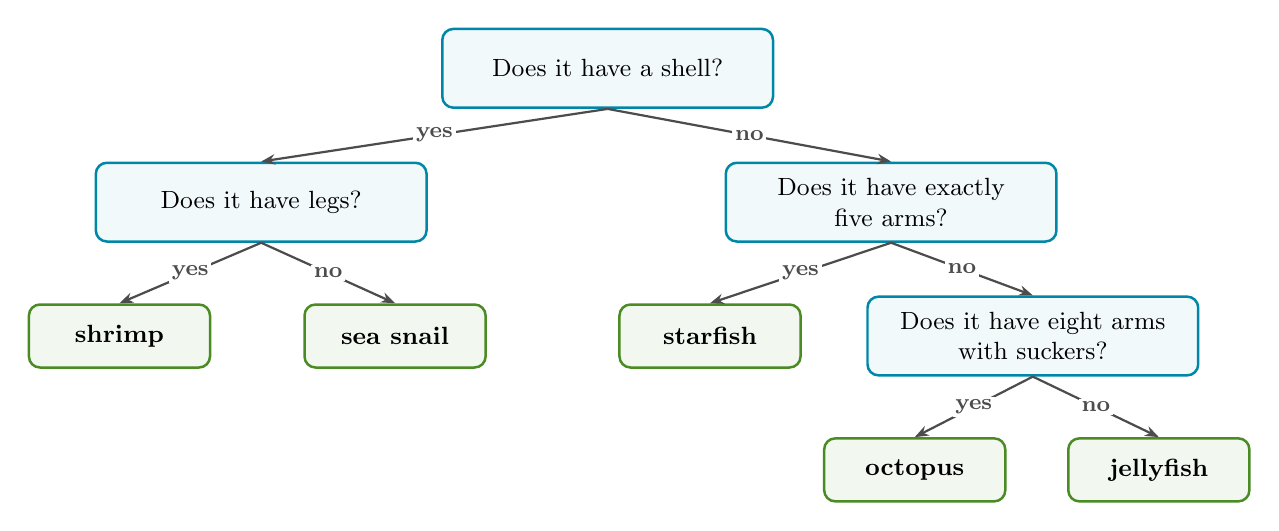
\begin{tikzpicture}[x=1cm, y=1cm,
    kq/.style={qbox, minimum width=4.2cm, minimum height=1.0cm},
    kn/.style={nbox, minimum width=2.3cm, minimum height=0.8cm, font=\small\bfseries}]
  \node[kq] (q1) at (0,0) {Does it have a shell?};
  \node[kq] (q2) at (-4.4,-1.7) {Does it have legs?};
  \node[kq] (q3) at (3.6,-1.7) {Does it have exactly\\five arms?};
  \node[kn] (shr) at (-6.2,-3.4) {shrimp};
  \node[kn] (sna) at (-2.7,-3.4) {sea snail};
  \node[kn] (sta) at (1.3,-3.4) {starfish};
  \node[kq] (q4) at (5.4,-3.4) {Does it have eight arms\\with suckers?};
  \node[kn] (oct) at (3.9,-5.1) {octopus};
  \node[kn] (jel) at (7.0,-5.1) {jellyfish};
  \draw[br] (q1.south) -- node[yn] {yes} (q2.north);
  \draw[br] (q1.south) -- node[yn] {no} (q3.north);
  \draw[br] (q2.south) -- node[yn] {yes} (shr.north);
  \draw[br] (q2.south) -- node[yn] {no} (sna.north);
  \draw[br] (q3.south) -- node[yn] {yes} (sta.north);
  \draw[br] (q3.south) -- node[yn] {no} (q4.north);
  \draw[br] (q4.south) -- node[yn] {yes} (oct.north);
  \draw[br] (q4.south) -- node[yn] {no} (jel.north);
\end{tikzpicture}
\end{minipage}

\vspace{10pt}
\noindent\begin{minipage}{\textwidth}
\noindent Mr Bowen finds five animals. Follow the key. Write each one's \textbf{name}.
P is done for you.

\vspace{2pt}
{\renewcommand{\arraystretch}{1.35}%
\noindent\begin{tabularx}{\textwidth}{|c|L|C{3.2cm}|}
  \hline
  & \textbf{What Mr Bowen sees} & \textbf{Name} \\ \hline
  P & No shell. Eight soft arms, each with two rows of suckers. & \tl{octopus} \\ \hline
  Q & A thin shell. Ten legs and two long feelers. & \\ \hline
  R & No shell. A soft round top, like an umbrella. Many tentacles. & \\ \hline
  S & No shell. Five arms in the shape of a star. & \\ \hline
  T & A round, curly shell. It moves on one soft foot. No legs. & \\ \hline
\end{tabularx}}
\end{minipage}

% -- C2 ---------------------------------------------------------------------
% Build the key from B1. The frame forces a 3-3 first split: 3 = 1 + 2,
% 2 = 1 + 1, so five questions for six names. One answer is in the key.
\clearpage
\qhead{C2}{Build a dichotomous key: the six animals}

\noindent\begin{minipage}{\textwidth}
\begin{remember}[Remember from Science 4.5]
  \textbf{To build a key:} \ \textbf{1} Split the organisms into two groups. \
  \textbf{2} Split each group into two again. \
  \textbf{3} Stop when each one has its own name.
\end{remember}

\noindent Build a key for the \key{six animals in the B1 table}. Use the table: every
question uses one of your B4 questions or another good one.
Your \textbf{first} question must split the six into \textbf{3 and 3}.
Write a question in each blue box and a name in each green box.

\vspace{8pt}
\centering
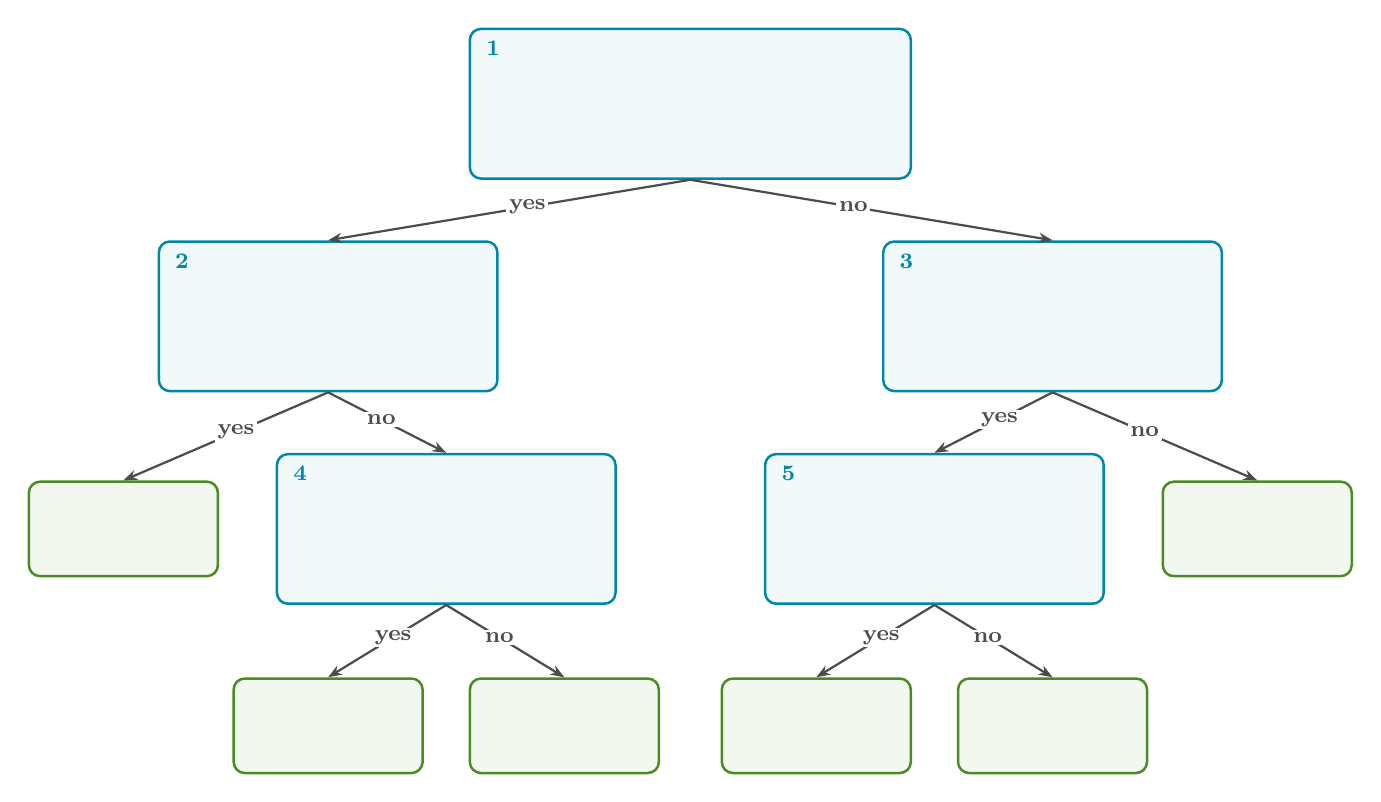
\begin{tikzpicture}[x=1cm, y=1cm]
  \node[qbox, minimum width=5.6cm] (q1) at (0,0) {};
  \node[font=\footnotesize\bfseries, text=cbteal, anchor=north west] at
    ($(q1.north west)+(0.1,-0.05)$) {1};
  \node[qbox] (q2) at (-4.6,-2.7) {};
  \node[font=\footnotesize\bfseries, text=cbteal, anchor=north west] at
    ($(q2.north west)+(0.1,-0.05)$) {2};
  \node[qbox] (q3) at (4.6,-2.7) {};
  \node[font=\footnotesize\bfseries, text=cbteal, anchor=north west] at
    ($(q3.north west)+(0.1,-0.05)$) {3};
  \node[nbox, minimum width=2.4cm] (n1) at (-7.2,-5.4) {};
  \node[qbox] (q4) at (-3.1,-5.4) {};
  \node[font=\footnotesize\bfseries, text=cbteal, anchor=north west] at
    ($(q4.north west)+(0.1,-0.05)$) {4};
  \node[qbox] (q5) at (3.1,-5.4) {};
  \node[font=\footnotesize\bfseries, text=cbteal, anchor=north west] at
    ($(q5.north west)+(0.1,-0.05)$) {5};
  \node[nbox, minimum width=2.4cm] (n6) at (7.2,-5.4) {};
  \node[nbox, minimum width=2.4cm] (n2) at (-4.6,-7.9) {};
  \node[nbox, minimum width=2.4cm] (n3) at (-1.6,-7.9) {};
  \node[nbox, minimum width=2.4cm] (n4) at (1.6,-7.9) {};
  \node[nbox, minimum width=2.4cm] (n5) at (4.6,-7.9) {};
  \draw[br] (q1.south) -- node[yn, pos=0.45] {yes} (q2.north);
  \draw[br] (q1.south) -- node[yn, pos=0.45] {no} (q3.north);
  \draw[br] (q2.south) -- node[yn, pos=0.45] {yes} (n1.north);
  \draw[br] (q2.south) -- node[yn, pos=0.45] {no} (q4.north);
  \draw[br] (q3.south) -- node[yn, pos=0.45] {yes} (q5.north);
  \draw[br] (q3.south) -- node[yn, pos=0.45] {no} (n6.north);
  \draw[br] (q4.south) -- node[yn, pos=0.45] {yes} (n2.north);
  \draw[br] (q4.south) -- node[yn, pos=0.45] {no} (n3.north);
  \draw[br] (q5.south) -- node[yn, pos=0.45] {yes} (n4.north);
  \draw[br] (q5.south) -- node[yn, pos=0.45] {no} (n5.north);
\end{tikzpicture}
\end{minipage}

% -- C3 ---------------------------------------------------------------------
% Most keys send the elephant to the water buffalo (or the sun bear): no
% scales, four legs, babies, heavy. The fix is a sixth question.
\vfill
\qhead{C3}{A new animal}

\noindent\begin{minipage}{\textwidth}
\noindent Mr Bowen visits a national park and sees an \textbf{Asian elephant}:
covered in thin hair, 4 legs, about 600 cm long, about 4000 kg, babies (1 at a time).

\vspace{4pt}
\begin{enumerate}[label=(\alph*), itemsep=8pt, topsep=2pt]
  \item Use \textbf{your} C2 key on the elephant. Which name does your key give?
        \ \blank[3.4cm]
  \item Is the name right? Why does this happen? Answer in a full sentence.
        \qlines{3}
  \item Write \textbf{one} new good key question that splits the elephant from that
        animal. Use a number if you can.
        \qlines{2}
\end{enumerate}
\end{minipage}

% -- C4 ---------------------------------------------------------------------
\clearpage
\qhead{C4}{Check your key}

\noindent\begin{minipage}{\textwidth}
\noindent\textbf{(a)} Test your C2 key on the \textbf{king cobra}. Start at box 1 and
draw over its path with a \textbf{pencil}, all the way to its name. Does it end on
\emph{king cobra}? \quad yes \sep no
\end{minipage}

\vspace{12pt}
\noindent\begin{minipage}{\textwidth}
\noindent\textbf{(b)} Why is your key a \key{dichotomous} key? Finish the sentence. \\[3pt]
\eng{``It is dichotomous because every question \ldots''}
\qlines{3}
\end{minipage}

\vspace{10pt}
\noindent\begin{minipage}{\textwidth}
\noindent\textbf{(c)} A \textbf{duck} is about \textbf{55 cm} long. Write one good key
question that splits the \textbf{kingfisher} from the duck. Use the B1 table. Which kind of
data does your question use?
\qlines{2}
\noindent Kind of data: \blank[4.0cm]
\end{minipage}

\vspace{14pt}
\noindent\begin{minipage}{\textwidth}
\noindent\textbf{(d)} Test your key on a \textbf{user}. Ask someone at home to use your
C2 key on the \textbf{pangolin}. Did they reach the right name? \quad yes \sep no \\[4pt]
Write their \textbf{feedback}: one question that was hard, and why. \\[3pt]
\eng{``Question \ldots\ was hard because \ldots''}
\qlines{4}
\end{minipage}

% ===========================================================================
% ANSWER KEY -- TEACHER COPY ONLY
% ===========================================================================
\ifkey
\clearpage

\hwsection[cbred]{Answer Key --- Teacher Copy}

\linespread{1.0}\selectfont
\setlist[enumerate]{itemsep=2pt, topsep=3pt, leftmargin=*}

\qhead[cbred]{A1}{Equivalent fractions}
\noindent (a) $\fr{6}{8}, \fr{9}{12}, \fr{15}{20}, \fr{30}{40}$ \quad
(b) $\fr{6}{15}, \fr{10}{25}, \fr{16}{40}, \fr{40}{100}$ \quad
(c) $\fr{12}{18}, \fr{4}{6}, \fr{2}{3}$ \quad
(d) $\fr{5}{7}, \fr{15}{21}, \fr{50}{70}$

\smallskip
\noindent{\small Each box in a row needs a different multiplier \emph{from the first
fraction}, not from its neighbour. The usual slip is (a) $\fr{9}{\bx}$ $\to$ 10 (``add
1 like the 8''), or keeping $\times 2$ along the row. (c) and (d) go down: a student
who cannot see $24 \div 2$ should be asked ``what number goes into 24 and 36?''. (d)
starts with $\div 7$, which most will miss; 49 is $7 \times 7$.}

\qhead[cbred]{A2}{Equal or not equal}
\noindent (b) $\neq$ ($3 \times 4 = 12$, not 9) \quad (c) $=$ ($\times 3$) \quad
(d) $=$ (both $\fr{2}{3}$) \quad (e) $\neq$ ($\fr{12}{16} = \fr{3}{4}$)

\smallskip
\noindent{\small (d) has no whole-number multiplier from 6 to 8, so expect $\neq$: the
reason is going \emph{down} to $\fr{2}{3}$ first, as (a) shows. (e) $\fr{12}{16}$ looks
like ``$\times 4$'' of $\fr{3}{4}$, and it is --- so it is not $\fr{2}{3}$.}

\qhead[cbred]{A3}{Change it both ways}
\noindent (a) $\mx{7}{1}{4}$ \quad (b) $\mx{7}{5}{6}$ \quad (c) $\mx{8}{4}{7}$ \quad
(d) $4$ \quad (e) $\fr{43}{8}$ \quad (f) $\fr{58}{9}$ \quad (g) $\fr{21}{2}$ \quad
(h) $\fr{47}{10}$

\smallskip
\noindent{\small (d) is the trap: $36 \div 9 = 4$ remainder 0, so the answer is the
whole number 4, not $\mx{4}{0}{9}$. In (e)--(h) the error is $5 \times 3 + 8$ (multiplying by the numerator) or forgetting
to add: $5 \times 8 = 40$, so $\fr{40}{8}$. (c) needs $7 \times 8 = 56$; a student who
writes $\mx{8}{3}{7}$ has slipped on $60 - 56$.}

\qhead[cbred]{A4}{Which is bigger?}
\noindent (a) $\fr{19}{4} = \mx{4}{3}{4}$, bigger than $\mx{4}{1}{2} = \mx{4}{2}{4}$
\quad (b) equal: $\fr{11}{3} = \mx{3}{2}{3}$ \quad
(c) $\mx{4}{1}{3} = \fr{13}{3} = \fr{26}{6}$, bigger than $\fr{25}{6}$

\smallskip
\noindent{\small (a) needs $\fr{1}{2} = \fr{2}{4}$ too. (c) is the hardest item in
Section A: two steps (mixed $\to$ improper, then $\times 2$). ``25 is bigger than 13''
is the trap.}

\qhead[cbred]{A5}{Mr Bowen and the fractions}
\noindent (a)(i) $\fr{19}{6} = \mx{3}{1}{6}$ pizzas \quad (ii) $\fr{5}{6}$ of a pizza
($24 - 19 = 5$ slices) \quad (b) 11 times ($\mx{2}{3}{4} = \fr{11}{4}$)

\smallskip
\noindent{\small (a)(ii): expect $\fr{5}{24}$ (left of all the slices, not of one
pizza). The question says \emph{a pizza}; accept $\fr{5}{24}$ \emph{of the four pizzas}
only if they say so. (b) is A3 in disguise: count the quarters in $\mx{2}{3}{4}$.}

\qhead[cbred]{A6}{Mr Bowen's homework}
\noindent Row 1 wrong: he added 1 to the top and the bottom; $\fr{2}{3} = \fr{4}{6}$
(any equivalent). \quad Row 2 \textbf{right} ($= \mx{3}{1}{2}$ too). \quad
Row 3 wrong: he multiplied and did not add the 1; $\fr{16}{5}$. \quad
Row 4 wrong: he swapped the answer and the remainder; $\mx{5}{3}{4}$.

\smallskip
\noindent{\small Row 2 will be marked wrong by many because $\fr{2}{4}$ ``is not
finished''. It is equal, so it is right. Row 4: the giveaway is that $\fr{5}{4}$ is
improper inside a mixed number.}

\qhead[cbred]{A7}{Write the question}
\noindent{\small Check the conditions in order: a real thing cut into 4 equal pieces;
23 pieces; asks how many \emph{wholes}; the word \emph{whole}; a question mark. A model:
``A cake shop cuts each cake into 4 equal pieces. It sells 23 pieces. How many whole
cakes and what fraction of a cake is that?'' Watch for questions whose answer is 23 or
4 (they asked how many pieces).}

\qhead[cbred]{B1}{Six animals}
\noindent Legs: discrete. \ Length: continuous. \ Mass: continuous. \ Eggs or babies:
categorical. \ Eggs or babies at one time: discrete.
\quad (a) kingfisher, 40 g \quad (b) 3; $\fr{3}{6} = \fr{1}{2}$

\smallskip
\noindent{\small ``Number of'' is the count signal; ``(cm)'' and ``(kg)'' are the measure
signal. Expect ``eggs or babies'' as discrete from students who see the next row's
numbers.}

\qhead[cbred]{B2}{The hard ones}
\noindent (a) discrete \quad (b) continuous \quad (c) categorical \quad (d) continuous
\quad (e) discrete \quad (f) Wrong: mass is \emph{measured}, so it is continuous; 600 kg
is rounded --- the buffalo could be 600.4 kg.

\smallskip
\noindent{\small (b) and (d) are the ones that do not look like measuring: time and
distance are measured. (f) is the 6.1 shoe-size idea turned round: a whole number does
not make data discrete; counting does.}

\qhead[cbred]{B3}{Baby crocodiles}
\noindent (a) 3, 4, 5, 3, 1; total 16. \quad (b) No: longer than 27 cm are 27.1, 27.5, 27.8, 27.3, 28.3, 28.8, 28.1, 29.4 --- 8 out
of 16, which is half, not most.

\smallskip
\noindent{\small (b) is the critical-thinking item. 27.0 is \emph{not} longer than 27,
so the grouped table's 9 (27.0 and up) is the trap. A student who answers ``yes, 9 out
of 16'' has read the table well but not the words; give credit for the method, then
discuss ``longer than'' with the class.}

\qhead[cbred]{B4}{From data to a key question}
\noindent (b) e.g. Does it have more than 2 legs? / Does it have legs? \quad
(c) e.g. Is its mass more than 100 kg? \quad
(e) ``Heavy'' is different for everyone; e.g. ``Is its mass more than 10 kg?''

\smallskip
\noindent{\small Reject (c) answers with no number (``Is it heavy?'') --- that is (e).
Note that ``Does it have legs?'' is discrete even with no number in it: you count to 0.}

\qhead[cbred]{C1}{Use a key}
\noindent Q shrimp \quad R jellyfish \quad S starfish \quad T sea snail

\smallskip
\noindent{\small Expect T as ``starfish'' or R as ``octopus'' from students who jump to
a name without following the arrows. ``Exactly five'' is in the word help.}

\qhead[cbred]{C2 and C4}{Build the key}
\noindent One key that fits the frame (yes is always on the left):
1 Is its body covered in scales? Yes $\to$ 2, No $\to$ 3. \
2 Is its mass more than 20 kg? Yes: \textbf{Siamese crocodile}; No $\to$ 4. \
4 Does it have legs? Yes: \textbf{pangolin}; No: \textbf{king cobra}. \
3 Does it have 4 legs? Yes $\to$ 5; No: \textbf{kingfisher}. \
5 Is its mass more than 100 kg? Yes: \textbf{water buffalo}; No: \textbf{sun bear}.
\quad C4(a) for this key: box 1 yes, box 2 no, box 4 no. \quad C4(b): ``\ldots every
question has two answers (yes or no), so it branches into two.'' \quad C4(c): e.g. ``Is it longer
than 30 cm?'' (continuous); ``Does it have webbed feet?'' is good too (categorical: you
can see it).

\smallskip
\noindent{\small Other good first questions for 3 and 3: Does it lay eggs? (cobra,
kingfisher, crocodile). Students may write a question whose ``yes'' side has two
animals where the frame has one; accept a key that works if the arrows and names agree.
Check, in order: six different names, one per green box; every question is yes/no with
one answer from everyone (count, measure or see); the king cobra's path ends on its
name. Reject
``Is it big?'', ``Is it dangerous?'', ``Is it a bird?'' (naming the answer is not a key
question).}

\qhead[cbred]{C3}{A new animal}
\noindent (a) Usually \textbf{water buffalo} (or sun bear). \quad (b) No; a key can only
identify the organisms that are in it, and the elephant is not in it. \quad (c) e.g.
Is its mass more than 1000 kg? / Is it longer than 4 m? / Does it have a trunk?

\smallskip
\noindent{\small (c) with ``Is it bigger?'' is the 4.5 error again. ``Does it have a
trunk?'' is a good question (you can see it), even with no number.}
\fi

\end{document}
